% !TEX TS-program = pdflatex
% !TEX encoding = UTF-8 Unicode

% This is a simple template for a LaTeX document using the "article" class.
% See "book", "report", "letter" for other types of document.

\documentclass[11pt,twoside]{report} % use larger type; default would be 10pt

\linespread{1}
\renewcommand*\rmdefault{ptm}

\usepackage[utf8]{inputenc} % set input encoding (not needed with XeLaTeX)

%%% Examples of Article customizations
% These packages are optional, depending whether you want the features they provide.
% See the LaTeX Companion or other references for full information.

%%% PAGE DIMENSIONS
\usepackage{geometry} % to change the page dimensions
\geometry{a4paper} % or letterpaper (US) or a5paper or....
\geometry{
	margin=2.5cm,
} % for example, change the margins to 2 inches all round
% \geometry{landscape} % set up the page for landscape
%   read geometry.pdf for detailed page layout information

\usepackage{graphicx} % support the \includegraphics command and options

% \usepackage[parfill]{parskip} % Activate to begin paragraphs with an empty line rather than an indent

%%% PACKAGES
\usepackage{url}
\usepackage{booktabs} % for much better looking tables
\usepackage{array} % for better arrays (eg matrices) in maths
\usepackage{paralist} % very flexible & customisable lists (eg. enumerate/itemize, etc.)
\usepackage{verbatim} % adds environment for commenting out blocks of text & for better verbatim
\usepackage{subfig} % make it possible to include more than one captioned figure/table in a single float
\usepackage[final]{pdfpages}
% These packages are all incorporated in the memoir class to one degree or another...

%%% HEADERS & FOOTERS
\usepackage{fancyhdr} % This should be set AFTER setting up the page geometry
\pagestyle{fancy} % options: empty , plain , fancy
\renewcommand{\headrulewidth}{0pt} % customise the layout...
\lhead{\small Teaching Quantum Mechanics Using qCraft}\chead{}\rhead{\small Micha van den Enk, s1004654}
\lfoot[\small \today]{\small \thepage}
\cfoot{}
\rfoot[\small \thepage]{\small \today}

%%% SECTION TITLE APPEARANCE
\usepackage{sectsty}
\allsectionsfont{\sffamily\mdseries\upshape} % (See the fntguide.pdf for font help)
% (This matches ConTeXt defaults)

%%% RULE

\newcommand{\HRule}{\rule{\linewidth}{0.5mm}}

%%% BIBLIOGRAPHY

\usepackage{apacite}                           %bibliography in apa-style

%%% ToC (table of contents) APPEARANCE
\usepackage[nottoc,notlof,notlot]{tocbibind} % Put the bibliography in the ToC
\usepackage[titles,subfigure]{tocloft} % Alter the style of the Table of Contents
\renewcommand{\cftsecfont}{\rmfamily\mdseries\upshape}
\renewcommand{\cftsecpagefont}{\rmfamily\mdseries\upshape} % No bold!

\setcounter{secnumdepth}{-2}

%%% TABLES

\renewcommand{\arraystretch}{1.2}

\usepackage{afterpage}

\newcommand\blankpage{%
    \null
    \thispagestyle{empty}%
    \newpage}

%%% END Article customizations

%%% The "real" document content comes below...

\begin{document}

\begin{titlepage}

\begin{center}


% Upper part of the page

\includegraphics[width=1\textwidth]{./logo}\\[1cm]    

\textsc{\Large Bachelor Thesis}\\[0.5cm]
\textsc{\Large {[}201000166{]}}\\[0.5cm]


% Title
\HRule \\[0.4cm]
{ \huge \bfseries Teaching Quantum Mechanics Using qCraft}\\[0.4cm]

\HRule \\[1.5cm]

% Author and supervisor
\begin{minipage}{0.4\textwidth}
\begin{flushleft} \large
\emph{Author:}\\
Micha \textsc{van den Enk} \\
{[}s1004654{]} \\
\end{flushleft}
\end{minipage}
\begin{minipage}{0.4\textwidth}
\begin{flushright} \large
\emph{Supervisors:} \\
Dr. H. H. \textsc{Leemkuil} \\
Second \textsc{supervisor} \\
\end{flushright}
\end{minipage}

\vfill

% Bottom of the page
{\large \today}

\end{center}

\end{titlepage}

\afterpage{\blankpage}

\setcounter{tocdepth}{1}
\tableofcontents
\thispagestyle{fancy}
\newpage

\section{Preface}

%%% ANALYSIS

\section{The Generic Model}

\begin{figure}[h]
\centering
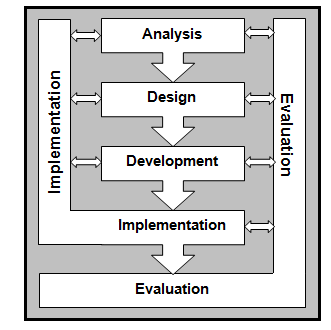
\includegraphics[width=0.7\textwidth]{genericmodel}
\caption{\footnotesize The generic model by \protect\citeA{genericmodel}\label{fig:genericmodel}}
\end{figure}

\chapter{Analyses}
\thispagestyle{fancy}

The first step of the Generic Model by \citeA{genericmodel} (see figure~\ref{fig:genericmodel} on page~\pageref{fig:genericmodel}) is Analysis. \citeA{smithragan} give an elaborated description of how to perform these analyses for instructional design. They distinguish three different kinds of analysis: analyzing the learner context, analyzing the learner and analyzing the learning task. The analysis of the learning context can provide the instructional needs and a description of the different factors influencing the instruction. The purpose of the learner analysis is the characterization of the end user of the instruction, which is in this case the middle school students. In the task analysis the test specifications are written, with which the content of the instruction can be established.These three analyses are executed in the following three chapters.

% Context Analysis

\section{Context Analysis}

A learning task always takes place in a certain learning context. In this case this is the middle school. It entails not only the place, but also the temporal and social environment \cite{smithragan}. The analysis of the learning context can provide the instructional needs and a description of the different factors influencing the instruction. With the instructional needs, the designer can establish the main learning goals for the instruction. The description of the learning environment can provide the learning opportunities and constraints which have to be taken into account for the instruction.

%needs assessment

\subsection{Needs Assessment}

The first goal of the need assessment is to investigate whether there exists a need for the instruction.  Without a need, it would be a waste of resources to develop the instruction \cite{smithragan}. Next to this, it is conducted to better specify the need for the instruction. In the context of instruction, the assessment often results in a learning goal, which is the main goal of the instruction. This main goal is needed to continue the rest of the analyses, because all other analyses are conducted in respect to this goal. The goal can also be used to construct the summative evaluation, because when this goal is achieved, the instruction has proved to be successful.

\citeA{smithragan} identify three different models for the needs assessment, namely the problem model, the innovation model and the discrepancy model (see figure~\ref{fig:needsassessment}). The problem model is used when there exists a problem in the current system which has to be solved. As can be seen in figure~\ref{fig:needsassessment}, this model is to be used as a prerequisite for the other two models for assessment. With this model, it is determined whether there really is a problem, whether the cause of the problem is related to emloyees' performance or learners' achievement, whether the solution to the problem is learning and whether instruction for these learning goals is currently offered. After the problem model, the needs assessment splits into the two other models. The innovation model is used when there is a new learning goal that the learners should achieve, and the discrepancy model is used when the already available instruction is not adequate to achieve the learning goal. The designer should choose one of these models for his needs assessment.

\begin{figure}[h]
\centering
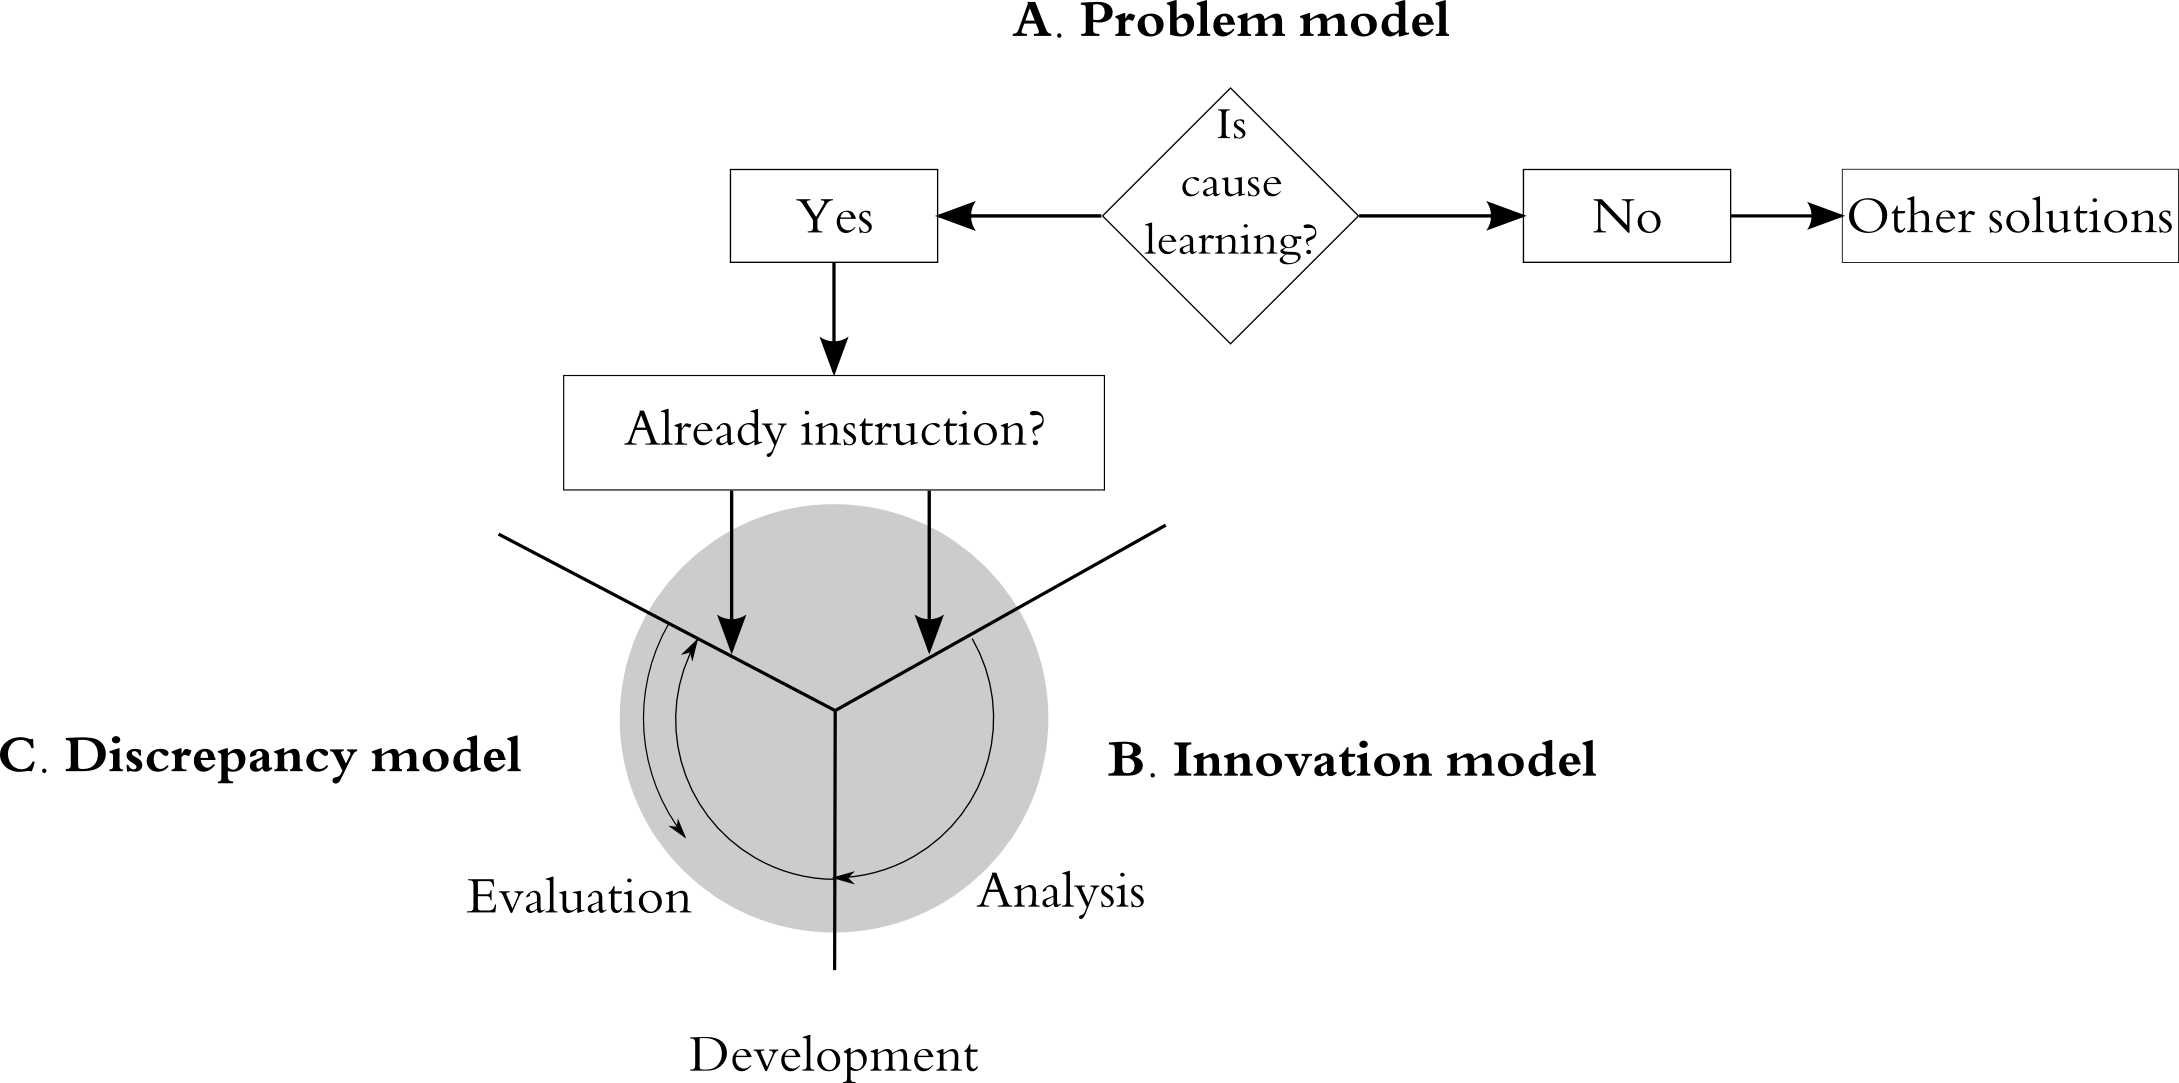
\includegraphics[width=\textwidth]{needsassessment}
\caption{\footnotesize The three sides of needs assessment \protect\cite{smithragan}\label{fig:needsassessment}}
\end{figure}

In the case of the instruction which will be constructed for this assignment, at first the problem model will be used to investigate the problem, and which of the two follow-up models should be used for the needs assessment.

\subsubsection{The problem}

In the Netherlands, quantum mechanics always used to be a topic which schools themselves could choose to teach or not to teach. The only skill students had to know for the Centraal Eindexamen (the national central exams at the end of high school) which comes close to quantum mechanics is to elucidate the photoelectric effect and the wave-particle duality, mentioned within point 20 under subdomain E3 \cite{eindexamen2015}. However, one of the changes in the Centraal Eindexamen of 2016 was the addition of domain F1, which is called Quantum world \cite{eindexamen2016}. For this subdomain the candidate has to be able to apply the wave-particle duality and the uncertainty principle of Heisenberg, and to explain the quantization of energy levels in some examples with a simple quantum physical model. In order to give all candidates a chance of passing this subdomain, schools have to alter their programs in order to meet the expectations of the Centraal Eindexamen.

However, when searching the internet using the search machine Google concerning the implementation of quantum mechanics in Dutch high schools, the quantity and the quality of the results are very low. There are also no results to be found in the Dutch papers. An example is the Dutch site http://www.quantumuniverse.nl/, where teachers can find a small amount of brief courses on fundamental quantum mechanics, and where the forums are very quiet with only 5 discussions, of which 4 are just started threads from the site administrator.

Upon finding this information, an expert was consulted to confirm this conjecture. The expert was researching the implementation of quantum mechanics on middle schools, and she also a first degree physics teacher. She stated that within her school there were no initiatives to bring this topic in their classrooms, and that their school was no exception as well.

The fact that next year domain F1 has to be fully implemented and taught to all vwo students who chose physics as an examination subject is therefore slowly turning into a sword of Damocles. This stresses the urgency for the development of new course material. Because it involves new instruction, the innovation model will be used for the second part of this needs assessment.

\subsubsection{The innovation}

The nature of the innovation lies within the change of the Centraal Eindexamen of 2016 in respect to the Centraal Eindexamen of 2015. The new additions within the domain Kwantumwereld outline the new goals of physics education in the Netherlands, and will be the ultimate goals for the students to achieve, and therefore be the ultimate learning goals for the students to achieve. This results in the following learning goals \cite{eindexamen2016}:

The candidate can:
\begin{itemize}
\item describe quantum phenomena in terms of the enclosure of a particle:
\begin{itemize}
\item estimate whether quantum phenomena are to expected by comparing the debroglie-wavelength with the order of largeness of the enclosure of the particle;
\item apply the uncertainty principle of Heisenberg;
\item describe the quantum model of the hydrogen atom and calculate the possible energies of the hydrogen atom;
\item describe the quantum model of a particle in a one-dimensional energy well and calculate the possible energies of the particle;
\item Bohr radius, zero-point energy.
\end{itemize}
\item describe the quantum-tunnel effect with a simple model and indicate how the chance of tunneling depends on the mass of the particle and the height and width of the energy-barrier,
\begin{itemize}
\item minimal in the contexts of: Scanning Tunneling Microscope, alpha-decay.
\end{itemize} 
\end{itemize}

These goals, however, cannot be reached during the instruction developed within the instruction, because of time constrains. Instead, the instruction will focus itself only explaining the three core principles of quantum mechanics, which are observer-dependency, superposition and entanglement. Without a thorough understanding of these principles, further elaboration is futile, because then a student will not be able to understand the uncertainty principle of Heisenberg, or the quantum-tunnel effect, and these are fundamental for even more advanced topics on quantum mechanics. So the goals of this innovation will be:

The candidate can:
\begin{itemize}
\item describe what is meant by observer-dependency;
\item describe the position of a quantum particle when it is in superposition;
\item describe what happens to the position of a set of entangled quantum particles.
\end{itemize}

%learning environment

\subsection{Learning Environment}

The learning environment description is the other major component of the learning context analysis \cite{smithragan}. The description contains information of all the external factors influencing the instruction. These are the mediators of the instruction, the already existing curricula which takes place in the environment, the available equipment available on the location of the instruction, the characteristics of the facilities at the location of the instruction, the characteristics of the organization in which the instruction will take place, and the philosophies and taboos of the larger community in which this organization exists.

For most teachers, quantum mechanics is a new subject to teach. However, a first degree teacher training \cite{leraarnatuurkundemaster} does encompass quantum mechanics, so the teachers should be familiar to the domain. Whether the teachers are familiar to the three principles is unclear at this moment, and would be an important aspect of implementation of this innovation. It should be investigated whether teachers already have sufficient knowledge on the topic, or need further instruction to use the innovation.

When implementing the instruction, the placing within the already existing curriculum is also important, because the instruction depends on prerequisites from other elements of the curriculum. The main prerequisite is knowledge of Bohr his atom model, because the different particles within this model are the particles on which quantum mechanics apply. This knowledge is teached in Domain E from the centraal eindexamen \cite{eindexamen2016}, and because of the prerequisite, it is of upmost importance that this instruction is placed after Domain E in the exisiting curriculum.

Another important aspect is the method of delivery \cite{smithragan}. If the instruction is delivered by traditional methods like books, teachers are already used to it and don't need further instruction. If the instruction is delivered otherwise however, it should be a part of the implementation to instruct the teachers how to use the technology. Another key element would be the available technology. If computers or tablets are used for the instruction, it should be investigated whether the available technology on the school is sufficient.

Finally, it is important to investigate whether the instruction fits in with the mission and vision of the school, and also the philosophies and taboos that the teachers hold. Therefore, it is advized to find these discrepancies by the means of interviews, in which the school board is asked about their mission and vision, and the teachers about their personal believes in regard to quantum mechanics.

In any case, this assignment does not look into the implementation of the instruction yet, so these factors have to be looked closer at when embedding the instruction in the context of a specific school.

% Learner analysis

\section{Learner Analysis}

The second analysis is that of the learners \cite{smithragan}. The purpose of this analysis is the characterization of the end user of the instruction, which is in this case the middle school students. For this analysis it is important to determine the similarities and differences between the learners. \citeA{smithragan} provide a list of factors which play a role in designing the instruction. They catagorize these factors with a ${2 \times 2}$ matrix (see table~\ref{tab:learneranalysis}), creating the catagories stable similarities, stable differences, changing similarities, and changing differences.

\begin{table}[h]
\begin{center}
\begin{tabular}{| l | l | l |}
\hline
 & \textbf{Similarities} & \textbf{Differences} \\ \hline
\textbf{Stable} & Stable similarities & Stable differences \\ \hline
\textbf{Changing} & Changing similarities & Changing differences \\ \hline
\end{tabular}
\end{center}
\caption{\footnotesize The four catagories of Learner Characteristics \protect \cite{smithragan} \label{tab:learneranalysis}}
\end{table}

%stable similarities

\subsection{Stable Similarities}

The stable similarities are the similarities between the members of the target audience which do not change. \citeA{smithragan} mention three types of stable similarities, namely the sensory capabilities, the information processing, and the types and conditions of learning.

Because of the young age of the target audience (17-18 years), the sensory capabilities are still high. It would make sense to stimulate the students by using both visual and auditory cues. On the other hand, according to information processing theories like Cognitive Load Theory \cite{smithragan}, it is important to also work with the constrains of the working memory. Therefore, it would be important to use the visual and auditory cues in a constructive way, without it being distractive from the learning content. \citeA{smithragan} mention a couple of strategies to decrease the cognitive load, for example off-loading, segmenting and weeding.

Which specific types and conditions of learning exist for the target demographic within the context of quantum mechanics will be researched during the literature research.

%stable differences

\subsection{Stable Differences}

There are also aspects of the members from the target audience which will not change which vary among these members. \citeA{smithragan} state them to be aptitudes, styles, traits and group membership factors.

The first of these aspects, aptitude, refers to the readiness or facility to learn or achieve. It is true that humans chosen by random sampling will probably differ among themselves in aptitude, also depending on the task or topic which they are assessed on. However, in the context of this assignment, only 6 vwo students which have chosen physics as an exam subject have to be considered. Because the group is so specific, their aptitude towards the subject of quantum mechanics can already be predicted to be relatively high. Another feature of this group is that they can be predicted to score high on assessments measuring logical/mathematical intelligence \cite{intelligences}, which is the type of intelligence required most in the context of learning quantum mechanics.

This analysis won't go into the different cognitive styles, psychosocial traits, or gender, ethnicity and racial groups. First of all, these are dependent on the place of implementation and the specific target audience. Next to this, the group membership factors are not relevant for this topic, for they are all personal aspects and do not relate to the field of quantum mechanics.

%changing similarities

\subsection{Changing Similarities}

\paragraph{Intellectual development processes}

\paragraph{Language development processes}

\paragraph{Psychosocial development processes}

\paragraph{Moral development processes}

\paragraph{Other development processes}

%changing differences

\subsection{Changing Differences}

\paragraph{Intellectual development state}

\paragraph{Other development state}

\paragraph{General prior learning}

\paragraph{Specific prior learning}

% Task analysis

\section{Task Analysis}

The final step is analyzing the learning task \cite{smithragan}. In this analysis the goals from the needs assessment during the analysis of the learning context have to be translated to test specifications, with which the content of the instruction can be established. In order to achieve these test specifications, first the type of learning has to be established. Having this established, the information-processing analysis can be conducted. Every type of learning has its own kind of information-processing analysis. \citeA{dance} provides a clear conceptual understanding of quantum teleportation, and will therefore be used to conduct this information-processing analysis. The next step is the prerequisite analysis. The outcome of this has to correspond to the outcome of the learner analysis. Finally, the learning objectives can be written, which form the test specifications. Every learning objective has to contain a description of the terminal behaviour or actions that will demonstrate learning, a description of the conditions of demonstration of that action and a description of the standard or criterion \cite{smithragan}. Every learning objective will fall into a category of Bloom his taxonomy of learning objectives \cite{bloom}, and will use appropriate action verbs. Most learning objectives within will be knowledge objectives, because there is a lot of new knowledge which has to be provided and it forms the basis for all other objectives. There will be no or very few synthesis and evaluation objectives, because these objectives would take too much time within the instruction to achieve to be feasible to use.

\subsection{Learning goal}

\subsection{Types of learning}

\subsection{Information-processing analysis}

\subsection{Prerequisite analysis}

\subsection{Learning objectives}

\subsection{Test specifications}

% Theoretic Framework

\chapter{Theoretic Framework}
\thispagestyle{fancy}

%%% DESIGN

\chapter{Design}
\thispagestyle{fancy}

%%% DEVELOPMENT

\chapter{Development}
\thispagestyle{fancy}

%%% FORMATIVE EVALUATION

\chapter{Formative Evaluation}
\thispagestyle{fancy}

\bibliographystyle{apacite}
\bibliography{references}

\end{document}
